\section{Exercise five}

Consider a server architecture composed of three main components: CPU, memory, and hard drive.
Each component has a constant failure rate of $\frac{1}{64}$, $\frac{1}{58}$ and $\frac{1}{28}$ per year, respectively, and failures are assumed to be independent events.
\begin{enumerate}
    \item Visualize the reliability block diagram of the server architecture.
    \item Calculate the mean time to failure for the server.
    \item Determine the reliability of the server over a three-year mission.
\end{enumerate}

\subsection*{Solution}
\begin{enumerate}
    \item The reliability block diagram of the server architecture is depicted below:
        \begin{figure}[H]
            \centering
            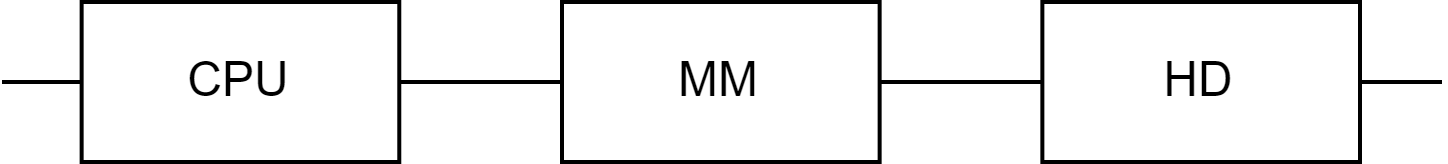
\includegraphics[width=0.5\linewidth]{images/server.png}
        \end{figure}
        Given that the components are in series, the total reliability is the sum of the reliabilities of each component:
        \[R(t)=R_{CPU}(t)+R_{memory}(t)+R_{hard\:disk}(t)=e^{-\lambda_{CPU}t}+e^{-\lambda_{memory}t}+e^{-\lambda_{hard\:disk}t}\]
    \item As the components are in series, the total failure rate is the sum of individual failure rates:
        \[\lambda_{tot}=\lambda_{CPU}+\lambda_{memory}+\lambda_{hard\:disk}=\dfrac{1}{64}+\dfrac{1}{58}+\dfrac{1}{28}=\dfrac{891}{12992}\]
        The mean time to failure is the inverse of the total failure rate:
        \[\text{MTTF}_{tot}=\dfrac{1}{\lambda_{tot}}=\dfrac{1}{\frac{891}{12992}}=14.58 \text{ years}\]
    \item The reliability for a three-year mission is:
        \[R_{tot}(3\text{ years})=e^{-3\lambda_{tot}}=0.814\]
\end{enumerate}